\documentclass{article}%
\usepackage[T1]{fontenc}%
\usepackage[utf8]{inputenc}%
\usepackage{lmodern}%
\usepackage{textcomp}%
\usepackage{lastpage}%
\usepackage[head=40pt,margin=0.5in,bottom=0.6in]{geometry}%
\usepackage{graphicx}%
%
\title{\textbf{El Papa Francisco advierte sobre las habladurías: "Por la lengua comienzan las guerras"}}%
\author{EUROPA PRESS}%
\date{04/03/2019}%
%
\begin{document}%
\normalsize%
\maketitle%
\textbf{URL: }%
http://www.eluniversal.com/internacional/34674/el{-}papa{-}francisco{-}advierte{-}sobre{-}las{-}habladurias{-}por{-}la{-}lengua{-}comienzan{-}las{-}guerras\newline%
%
\textbf{Periodico: }%
EU, %
ID: %
34674, %
Seccion: %
internacional\newline%
%
\textbf{Palabras Claves: }%
NO\_TIENE\newline%
%
\textbf{Derecho: }%
2.1%
, Otros Derechos: %
\newline%
%
\textbf{\textit{Francisco ha destacado la importancia de quienes tienen responsabilidades educativas o de liderazgo, exhortándolos a ser conscientes de su delicado papel y a discernir siempre el camino correcto a se}}%
\newline%
\newline%
%
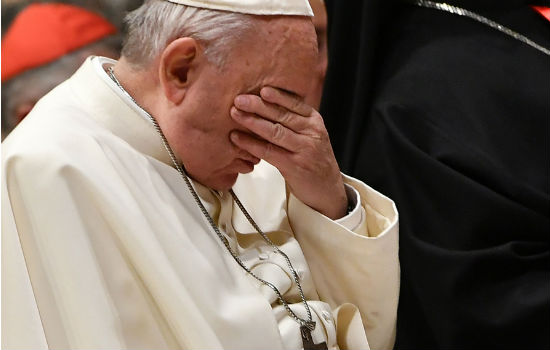
\includegraphics[width=300px]{EU_34674.jpg}%
\newline%
%
Roma.{-}El Papa ha advertido sobre las habladurías, que "destruyen" todos los ámbitos de la vida, como la familia, la escuela, el lugar de trabajo o la amistad: "Por la lengua comienzan las guerras", ha afirmado.%
\newline%
%
Durante su intervención en el Ángelus, Francisco ha destacado la importancia de quienes tienen responsabilidades educativas o de liderazgo, exhortándolos a ser conscientes de su delicado papel y a discernir siempre el camino correcto a seguir para guiar a las personas. cito Europa Press.%
\newline%
%
En este sentido ha exhorado a los fieles a no ser presuntuosos e hipócritas: "Muchas veces, todos lo sabemos, es más fácil o más cómodo ver y condenar las faltas y pecados de los demás, sin poder ver los propios con la misma lucidez".%
\newline%
%
El Pontífice ha subrayado que siempre escondemos nuestros defectos, "incluso los escondemos a nosotros mismos".%
\newline%
%
Ante esta actitud, el Papa ha recordado que existe la tentación de ser indulgente con uno mismo. Por eso "mientras observamos y corregimos las faltas de nuestro prójimo, también debemos ser conscientes de que nosotros tenemos faltas", ha manifestado.%
\newline%
%
"Si creo que no tengo defectos, no puedo condenar o corregir a los demás. Todos tenemos defectos: todos. Y debemos ser conscientes, y antes de condenar a otros debemos mirar dentro de nosotros mismos", subrayó Francisco.%
\newline%
%
\end{document}